%%%%%%%%%%%%%%%%%%%%%%%%%%%%%%%%%%%%%%%%%%%%%%%%%%%%%%%%%%%%%%%%%%%%%%%%%%%
%
% Plantilla para un artculo en LaTeX en espaol.
%
%%%%%%%%%%%%%%%%%%%%%%%%%%%%%%%%%%%%%%%%%%%%%%%%%%%%%%%%%%%%%%%%%%%%%%%%%%%

\documentclass[11pt,oneside,titlepage]{article}

% Esto es para poder escribir acentos directamente:
%\usepackage[latin1]{inputenc}
\usepackage[utf8]{inputenc}
\usepackage{makeidx}
\usepackage{multirow}
\usepackage{titlesec}
\usepackage{sectsty}
\usepackage{fncychap}
\usepackage{color}
\usepackage{comment}

% Esto es para que el LaTeX sepa que el texto est en espaol:
\usepackage[spanish]{babel}
\usepackage[right=3cm,left=3cm,top=2.5cm,bottom=2.5cm,headsep=1cm,footskip=2cm]{geometry}
\usepackage{graphicx}
% Paquetes de la AMS:
\usepackage{amsmath, amsthm, amsfonts}
\usepackage{fancyhdr}
\pagestyle{fancy}
\lhead{
\chead{
\rhead{\bfseries Informe Semanal de Actividades Realizadas }
\lfoot{\thepage}
\cfoot{}
\rfoot{Firma Supervisor: \_\_\_\_\_\_\_\_\_\_\_\_\_\_\_\_\_\_\_\_\_\_\_}
\renewcommand{\headrulewidth}{0.4pt}
\renewcommand{\footrulewidth}{0.4pt}
}}

%\pagestyle{headings}
%\pagestyle{myheadings}
%\markright{Informe Semanal de Actividades Realizadas}
\begin{document}
\title{Informe Semanal de Actvividades Realizadas}
\author{Nombre: Arturo Veras\\ 
	Supervisor: Claudio Torres\\
	Empresa: CCTVAL \\
Tipo de Práctica: Profesional}
%\date{\color{green}December 2005}
%\maketitle
%\setlength{\unitlength}{1 cm} %Especificar unidad de trabajo
\thispagestyle{empty}
\begin{picture}(0,1.5)
\put(0,0){
\includegraphics[width=2.7cm,height=2cm]{utfsm.jpg}}
\put(13,0){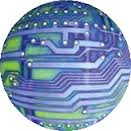
\includegraphics[width=2cm,height=2cm]{elo.jpg}}
\end{picture}
\\
\\
\begin{center}
\textbf{{\LARGE Universidad Técnica Federico Santa María}\\[0.5cm]
{\LARGE Departamento de Electrónica}}\\[4.25cm]
{\Large Informe de Práctica}\\[2.3cm]
{\LARGE \textbf{Centro Cient\'ifico Tecnol\'ogico de Valpara\'iso}}\\[3.5cm]
{\large Arturo Veras Olivos}\\[2cm]
Valparaiso - \today
\\
 {\large Versión 2.5}
\end{center}

%\newpage
%\tableofcontents
%\listoffigures % to produce list of figures
%\listoftables % to produce list of tables
%\newpage
\section*{Informe Semanal de Actividades Realizadas}
\begin{center}

\begin{tabular}{|r|l|}
\hline 
Nombre:  & Arturo Veras\\ 
\hline 
Supervisor & Claudio Torres \\ 
\hline 
Empresa: & CCTVAL \\ 
\hline 
Tipo de Práctica: & Profesional \\ 
\hline 
\end{tabular} 
\end{center}
\subsection*{Semana 1, del \textit{13/01/14 al 17/01/14}}
\begin{comment}
Tercera persona Él, Ella, Ello (del latín ille, illa, illud)
Se redacta en lenguaje formal y atemporal (no usar formas verbales en pasado simple)
Compró el periódico y se tomó un café.
\end{comment}

La primera tarea para esta semana es investigar formas de conectar una GPU (GT640 NVIDIA Graphic Card Unit) a una Raspberry Pi (Single Board Computer). Hay que tener encuentra que la interfaz de la tarjeta gr\'afica es PCIe 3.0 16x y la Raspberry Pi tiene el puerto GPIO (General-Purpose Input/Output) y USB 2.0 disponibles. Por lo tanto la primera estrategia es investigar si existe alg\'un dispositivo que haga de adaptador entre PCIe 16x y USB 2.0. 

Se propone conectar la GT640 a una tarjeta de desarrollo llamada \textbf{startKIT}, esta tarjeta posee una interfaz PCIe 1x y un puerto GPIO que se conecta facilmente a la Raspberry Pi. La idea es descartada porque no existen drivers para conectar una tarjeta de video, menos una NVIDIA, a este dispositivo. Además hay que desarrollar el driver para concetar la startKIT a la Raspberri Pi.

Otra idea que se propone es estudiar el funcionamiento de los adaptadores de PCIe a USB, particularmente el funcionamiento del chip el chip \textbf{MCS9901-CC} ya que, eventualmente, se puede diseñar una placa que hace la interfaz entre PCIe y USB en el modo que queremos.

La tercera idea que se propone es utilziar el adaptador de PCIe a Mini PCIe \textbf{PE4L-PM060}. La idea de este adaptador es utilizarlo en caso de que la Raspberry Pi no cuente con los requerimientos mínimos para conectarse a la GT640.

\subsection*{Semana 2, del 20/01/14 al 24/01/14}

Las tareas de esta semana consisten en seguir buscando otras alternativas ya que las
anteriores han sido descartas por el momento.

Se encuentra el chip \textbf{USB2380}, un controlador
PCIe 1.0 a USB 2.0. El problema es que para nuestro propósito, conectar la GT640 a través del puerto USB, se necesita
desarrollar un controlador propio. Por el momento creemos que esta solución esta
fuera de los objetivos principales, es más, aún no se posee información más
detallada sobre el desarrollo de dicha tarjeta. Otro problema que es que no
se sabe si podemos adquirir el dispositivo a tiempo para realizar pruebas ya que la compra se realiza en el extrangero.

Hasta la fecha no se ha encontrado un adaptador directo entre PCIe y USB, por lo tanto se decide por
estudiar la posibilidad de realizar una tarjeta que tenga ambas interfaces y que
cumpla con nuestros requerimientos. Las posibilidades son: \textbf{MCS990} PCIe
to 4-Port USB 2.0 Host Controller, este queda fuera porque no es posible realizar el adaptador,  y \textbf{USB2380} PCIe 1.0 to USB 2.0 controller aún se necesita buscar más información de como es el desarrollo del software controlador.

Miestras se contacta al desarrollador del chip USB2380 para más detalles se buscan otras alternavis para reemplazar la Raspberri Pi y que posean un slot PCIe. Se encuentra la tarjeta \textbf{SBC-A510 Single Board Computer}, esta tarjeta tiene un puerto mPCIe que podemos utilizar junto al adaptador \textbf{PE4L-PM060A}. Esta idea queda pendiente ya que la tarjeta es elevada y la idea principal es construir un dispositivo de bajo costo.

Finalmente para esta semana se concluye que no es posible la conexión de una tarjeta PCIe a la Raspberry Pi porque no cumple los requerimientos de hardware. A partir de la próxima semana la nueva estrategia será encontrar formas de que la GT640 actúe como un periférico USB con una conexión hot-plug.

\subsection*{Semana 3, del 27/01/14 al 31/01/14}

Se propone utilizar placa madre que tenga un puerto PCIe, el computador tendrá los requerimientos mínimos para que la GT640 funcione, el trabajo será conectar este computador a otro como periférico USB. 

Por otro lado se ha encontrador una solución similar muy parecida a lo que queremos desarrollar, se trata de una tarjeta desarrollo de llamada \textbf{Kayla}, básicamente es un computador pequeño que reune todas las características para trabajar con la tarjeta GT640 en HPC pero los costos son elevados y la GT640 se compra por separado.   

Mientras se estudia la posibilidad de conectar un computador como periferico USB, se sigue buscando alternativas que permitan conectar la GT640 de forma externa. Se encuentra un dispositivo la \textbf{USB3380-AB EVK-RC}, es una tarjeta de desarrollo que tiene la
version USB 3.0 del USB2380 chip previamente mencionado. Esta tarjeta posee un slot PCIe 1x y hasta el momento es justamente lo que estamos buscando. Nos ponemos en contacto para saber más detalles del software necesario para el funcionamiento.

Para el fin de la semana se tienen dos alternativas y cada una va por caminos diferentes. Primero se tiene la cotización del computador con los requerimientos mínimos y tenemos que estudiar la posibilidad de conexión USB como periférico a otro computador de forma hot-plug. Segundo es adquirir la USB3380-AB EVK-RC software necesario para nuestra aplicación.

Finalmente la idea de conectar la Raspberri Pi a la GT640 se descarto completamente ya que la Raspberry Pi no 
tiene la arquitectura necesaria para que CUDA, el software de desarrollo de las GPU de NVIDIA, funcione.

\subsection*{Semana 4, del 03/02/14 al 06/02/14}

Esta semana se realiza una revisión de todas las ideas previamente mencionadas. Se necesita una nueva estrategia porque el plan inicial comenzó a cambiar de rumbo. Con la alternativas previamente descartadas se decide comenzar de nuevo la investigación. Como aún no se tiene respuesta sobre el software controlador del USB3380-AB EVK-RC, se decide construir el computador de bajo costo, instalar la GT640 y CUDA. Por ahora nos centraremos en hacer funcionar el dispositivo a través del puerto USB de forma hot-plug. 

No queda claro aún si es posible conectar o no a través del puerto USB, normalmente la conexión se realiza Host-to-Device (master/slave) pero en este caso se pretende realizar una conexión Host-to-Host. El protocolo normalmente no permite este tipo de conexión.

Para esta semana aún no tenemos respuesta sobre USB3380-AB EVK-RC.

\subsection*{Semana 5, del 10/02/14 al 14/02/14}
\begin{comment}
lunes
- Ademas se realizó un estudio sobre como conectar el comptuador de una forma
plug and play, las opciones son utilizar el puerto Ethernet o, mejor aún,
realizar la conexión a trav\'es USB.

martes 
- Reunion con el profesor para ver el estado del proyecto. 3 ideas
  nuevas aparecieron.

miercoles 
- Contacto con un desarrollador de USB3380 para solicitar ayuda en el
  campo. 
- Estudio de RNDIS para conectar usb a usb, existe la posibilidad.

jueves 
- Estudio del funcionamiento de usb. Aprendi que podemos utilizar el
  computador como gadget y realizar la configuración recompilando el kernel y
  agregando los drivers.Mas detalles leer Linux Gadget Drivers
- Aún falta el cable. 
- Compilación del kernel para agregar los módulos. Estamos a la espera
  del cable USB macho macho.

viernes 
- Update del proyecto al profesor Claudio torres. 
 - compramos cable USB 3.0, estamos a la espera del envío.
\end{comment}


\subsection*{Semana 6, del 17/02/14 al 21/02/14}
\begin{comment}
lunes 
- Se adquirio el cable, se connecto pero no funciono. Se revisa si los
módulos estan compilados.  
-  Estudiar la posibilidad de crear un driver.  
- Se manda correo a lista-usb. Espera de respuesta.

martes -  No es posible conectar el cable usb entre PC. El hardware USB que
traen los PCI no es soportado por el driver linux gadget que es el encargado de
realizar esta conexión, 
- Hemos descartado la posibilidad de conectar PC to PC
con un cable simple.  Decidimos realizar la conexión a través de ethernet.

miercoles 
- NAAAAAAAAAAAAADAAAAAAAAAAAAAAA 

jueves 
- NNNNNNNNNNNNAAAAAAAAAAAADAAAAAAAaaaa 
viernes 
- NAAAAAAAAAAAAAAAADAAAAAAAAAAAa

\end{comment}

\subsection*{Semana 6, del 24/02/14 al 28/02/14}
\begin{comment}

lunes
- Se decide por comprar la tarjeta desarrollo USB33880 , Claudio Torres no
escucha nuestras advertencias de que hay que realiar el driver completamente y
aún asi decide comprarla. Francisco nos pide que le mandemos el valor para que
la Universidad realice la compra, el producto no es disponible. Mantemos al
tanto a Torres sobre el problema, no sabemos que hacer.  Por mientras cada uno
hace lo suyo.
-  

lunes
\end{comment}

\end{document}

